\secrel{Защитные цепи\ --- использование диода}

Диоды очень часто используемые компоненты, они бывают всех форм и размеров.

\begin{framed}\noindent
Диод\ --- электронный прибор, пропускающий ток только в одном направлении
\end{framed}

\includegraphics[height=0.3\textheight]{bcollis/vd/1N4004.jpg}
\includegraphics[height=0.3\textheight]{bcollis/vd/1N4007.jpg}
\includegraphics[height=0.3\textheight]{bcollis/vd/1N4148.jpg}

\noindent
\begin{tabular}{p{0.45\textwidth} p{0.45\textwidth}}
\noindent
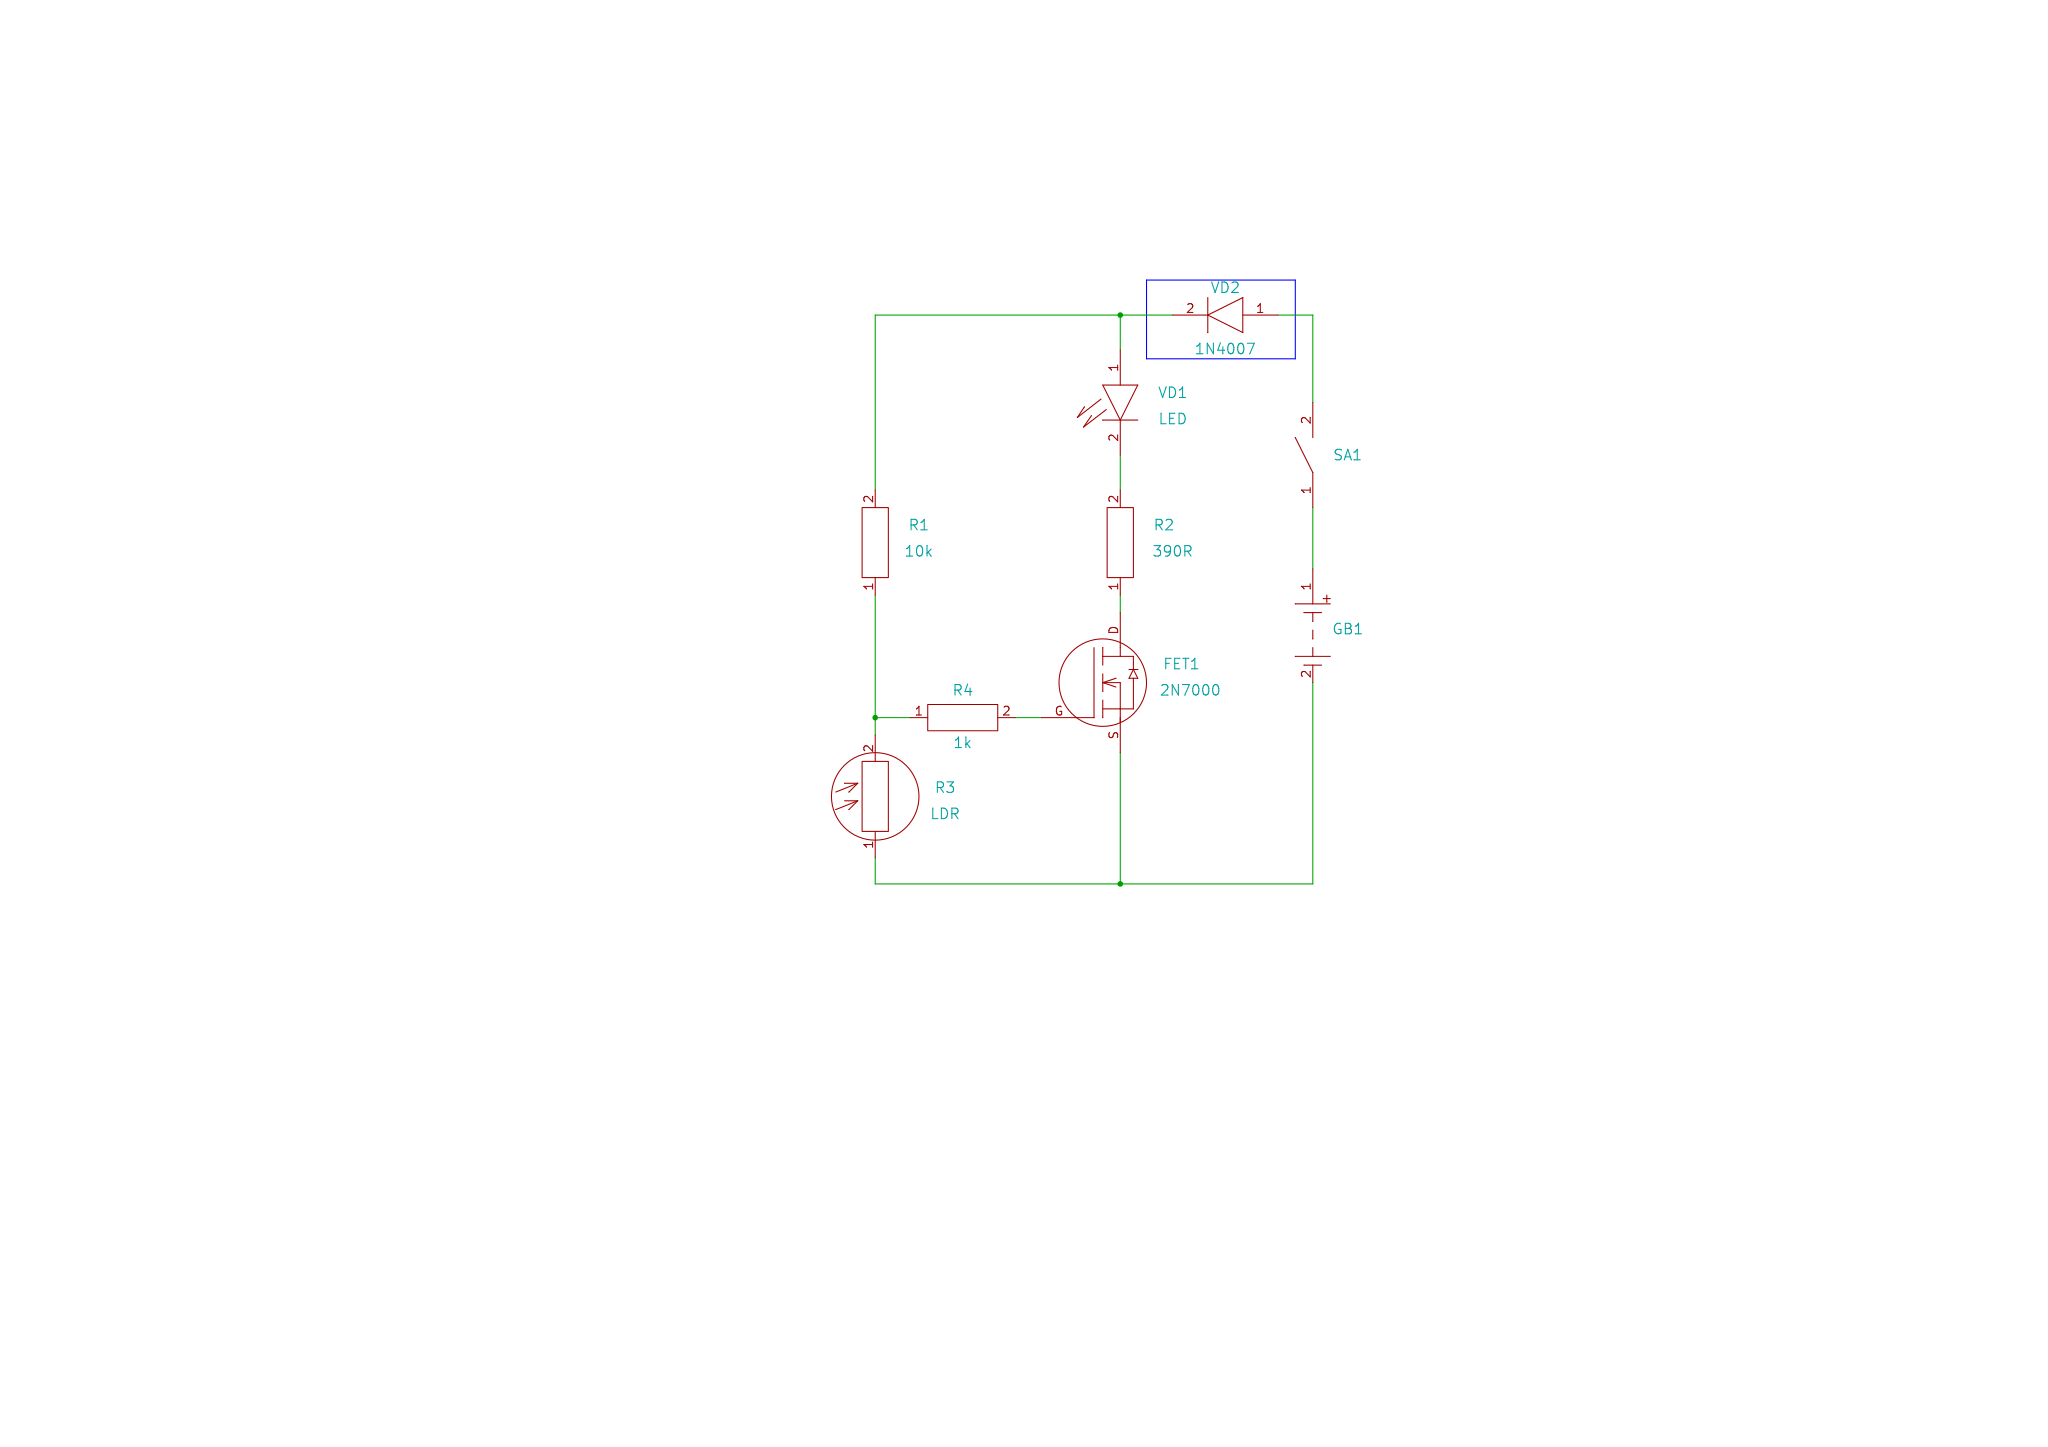
\includegraphics[width=0.45\textwidth]{bcollis/vd/vd.pdf}
&
\parbox[b]{0.5\textwidth}{
Основная характеристика диода\ --- то что ток течет только в одном направлении,
так что вы не можете его пустить в схеме в обратном направлении, и можете быть
уверены, что это работает. В этой модифицированной схеме питание подается от
батареи. Фраза "\term{цепь защищена диодом}"\ означает, что если батарея
ошибочно подключена в неправильной полярности, тока не будет, потому что диод
блокирует его. Это обычно используется в мастерской для защиты наших схем от
подачи питания обратной полярности.

Конечно, диод несовершенен, и если напряжение источника питания превысит
\termdef{максимальное обратное напряжение диода}{обратное напряжение диода}, то
диод будет сломан: обратный ток диода будет очень быстро расти, и сожгет диод.
1N4004 допускает обратное напряжение 400\,В. Диоды также могут проводить
определенный \termdef{ток в прямом направлении}{прямой ток диода}, иначе они
перегреваются и сгорают. 1N4004 имеет максимальный прямой ток 1\,А.
}
\\
\end{tabular}
